\begin{frame}[t]
\frametitle{Molecular Dynamics in NAMD}
  \begin{columns}
  \column{.8\textwidth}
  \begin{itemize}
    \item Collection of charged atoms, with bonds
    \begin{itemize}
      \item Newtonian mechanics
      \item Relatively small of atoms (100K – 10M)
    \end{itemize}
    \pause
    \item Calculate forces on each atom 
    \begin{itemize}
      \item Bonds
      \item Non-bonded: electrostatic and van der Waal’s
      \begin{itemize}
        \item Short-distance: every timestep
        \item Long-distance: using PME (3D FFT)
        \item Multiple Time Stepping : PME every 4 timesteps 
      \end{itemize}
    \end{itemize}
    \pause
    \item Calculate velocities and advance positions
    \item Challenge: femtosecond time-step, millions needed!
  \end{itemize}
  \pause
  \textcolor{red}{Collaboration with K. Schulten, R. Skeel, and coworkers}
  \column{.2\textwidth}
  \vfill
  \begin{center} 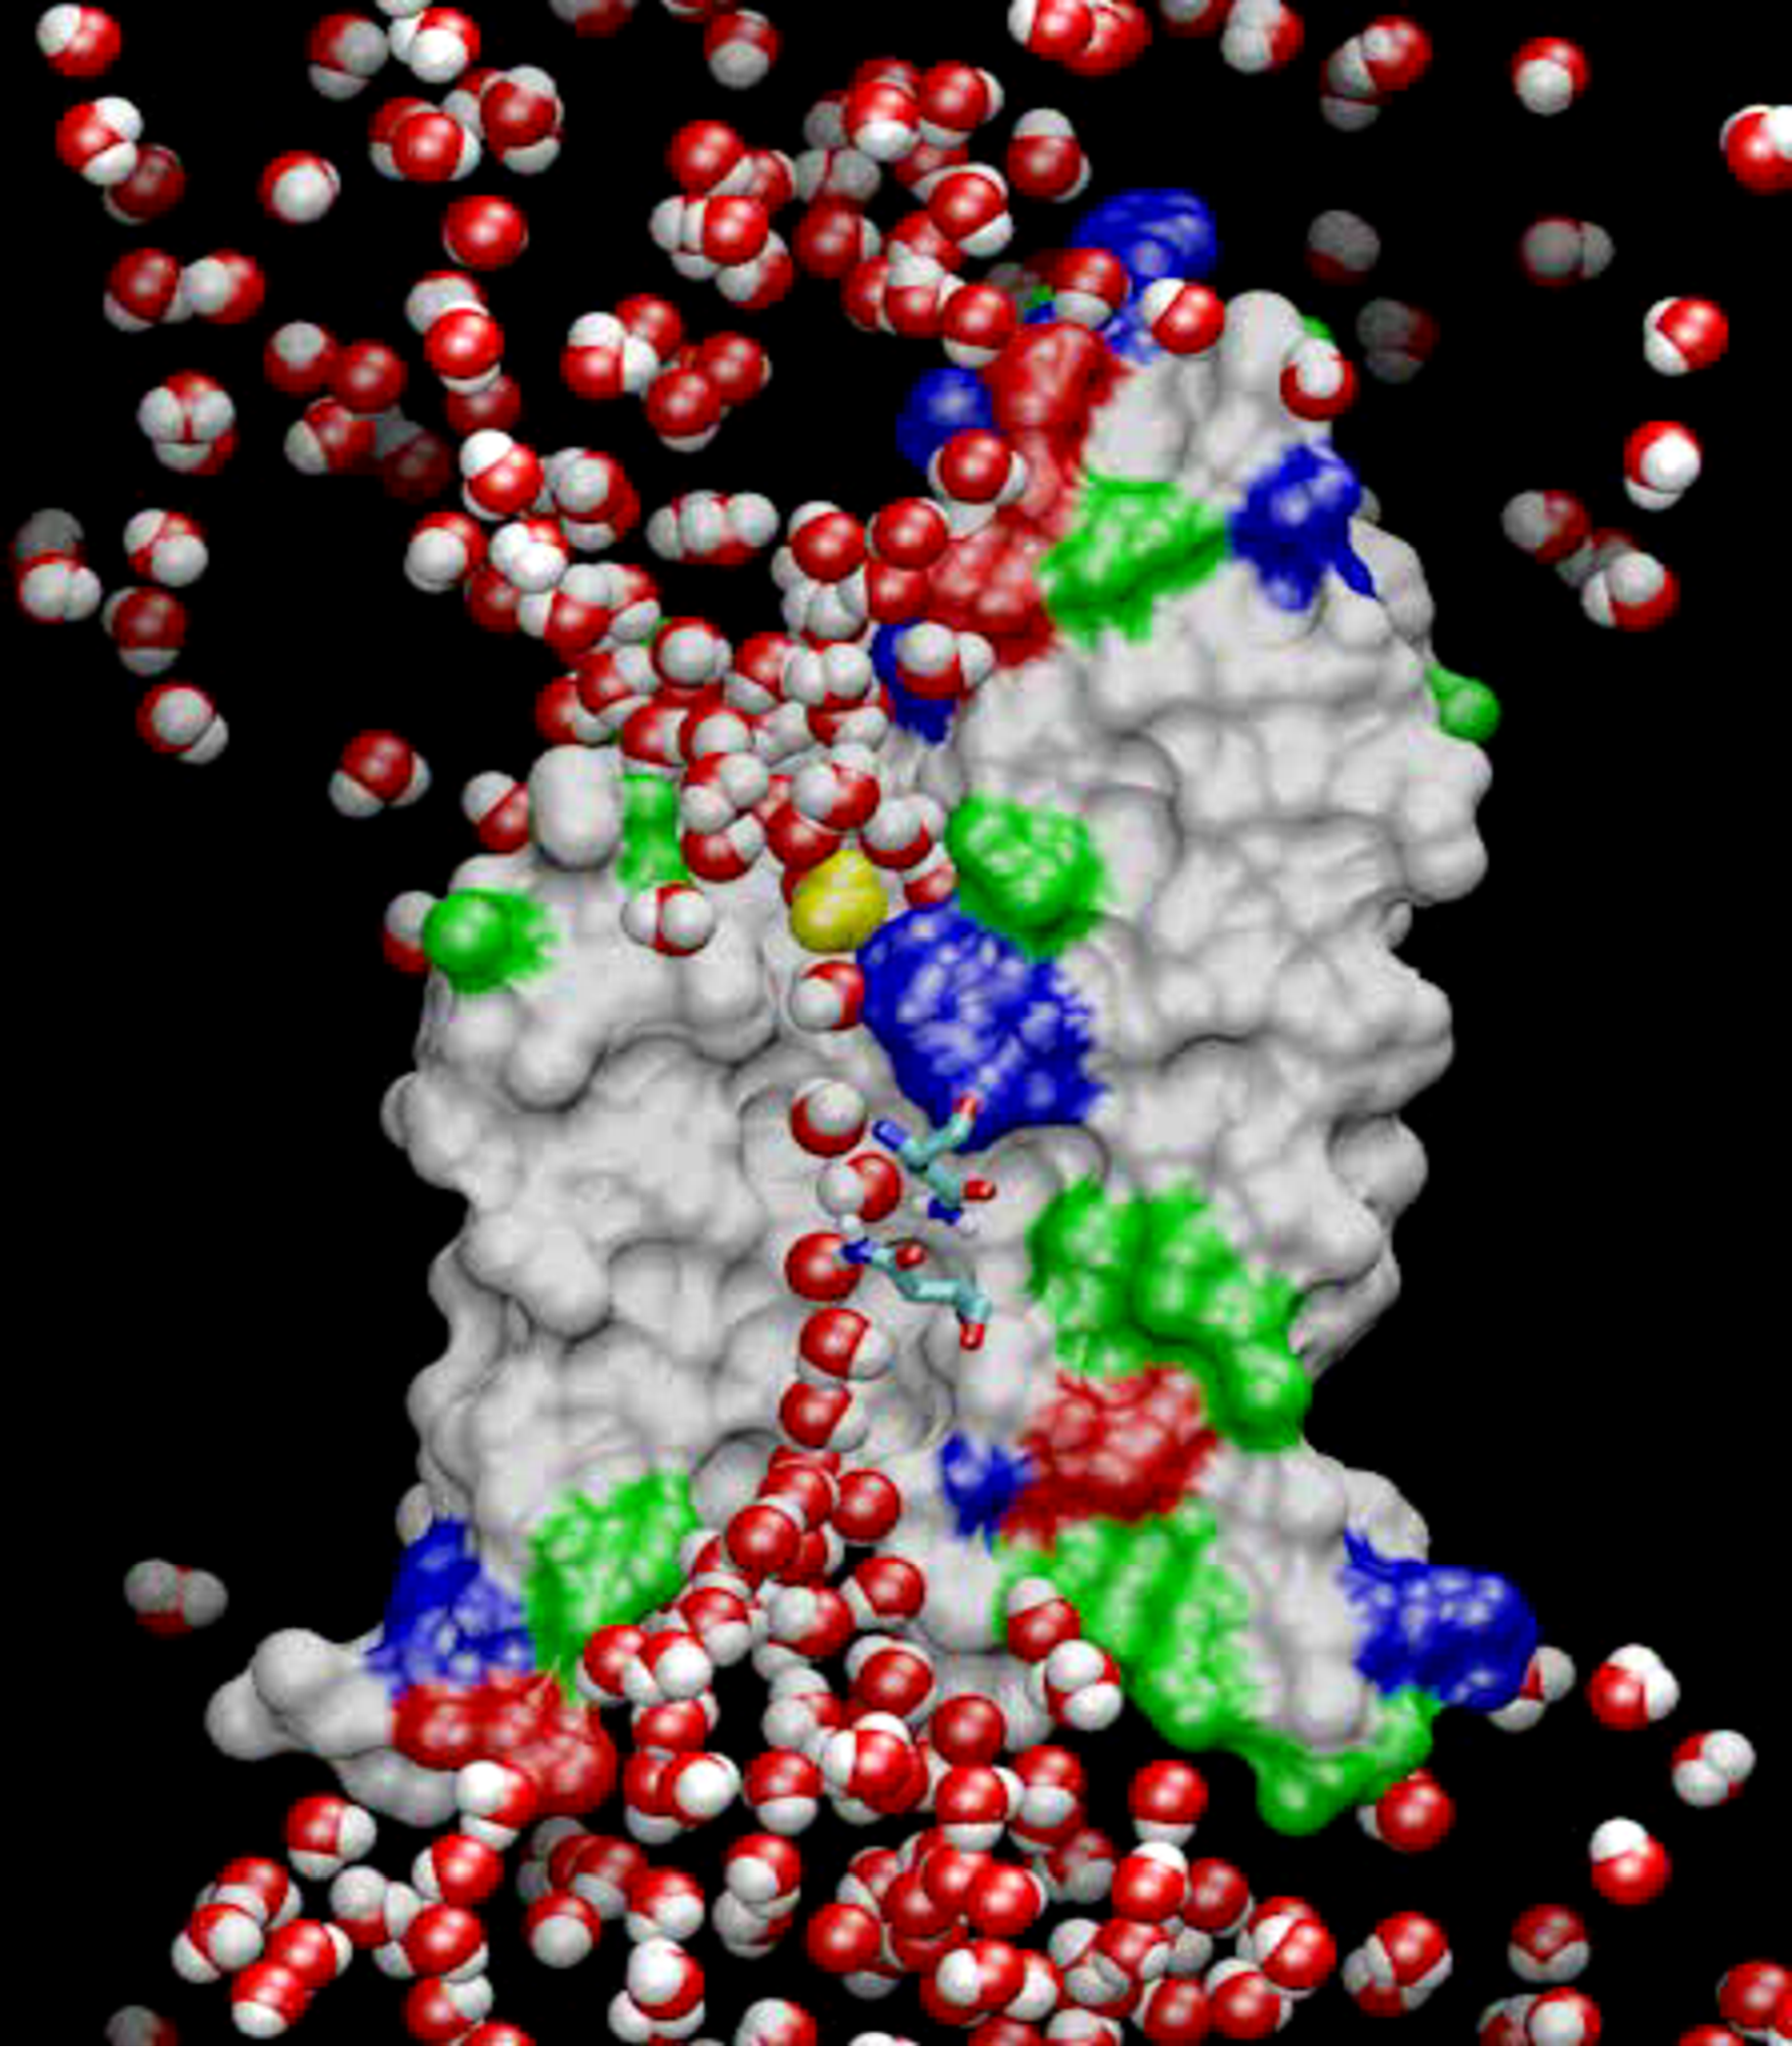
\includegraphics[width=\textwidth]{figures/namd.pdf} \end{center}
  \vfill
  \end{columns}
\end{frame}

\begin{frame}[t]
\frametitle{Spatial Decomposition Via Charm}
  \begin{columns}
  \column{.4\textwidth}
  \begin{center} 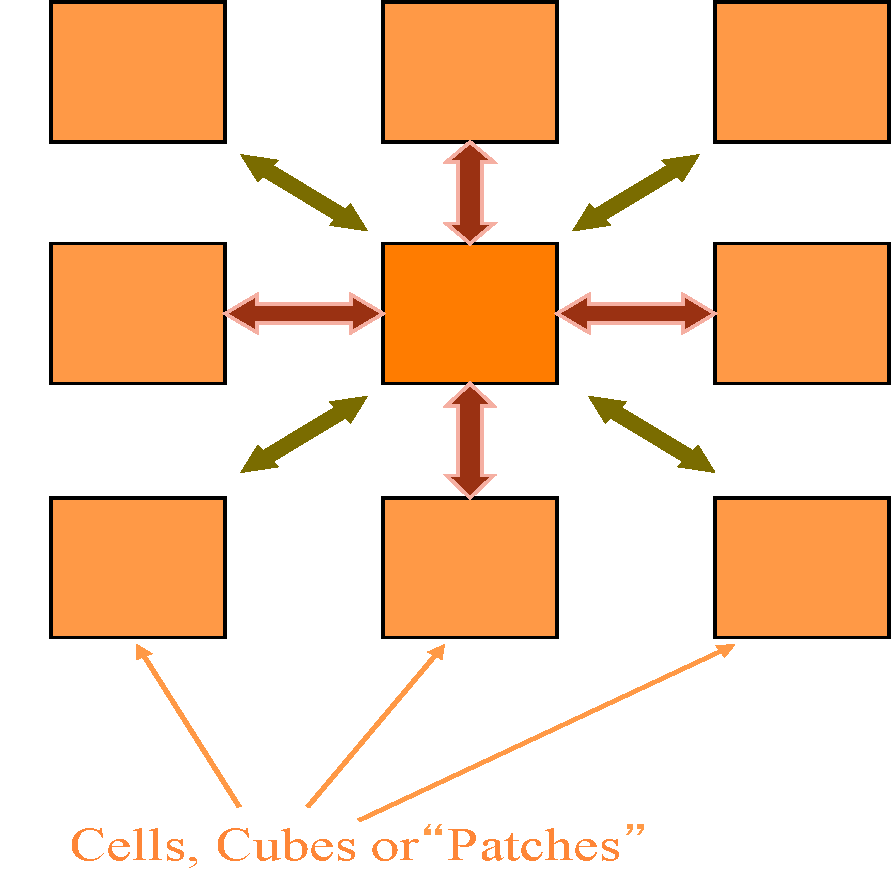
\includegraphics[width=0.8\textwidth]{figures/namd_decomp.pdf} \end{center}
  \column{.6\textwidth}
  \begin{itemize}
    \item Atoms distributed to cubes based on their location
    \pause
    \item Size of each cube :
    \begin{itemize}
      \item Just a bit larger than cut-off radius
      \item Communicate only with neighbors
      \item Work: for each pair of nbr objects
    \end{itemize}
    \item C/C ratio: O(1)
    \pause
    \item However: 
    \begin{itemize}
      \item Load imbalance
      \item Limited parallelism
    \end{itemize}
  \end{itemize}
  \pause
  \textcolor{red}{Charm++ is useful to handle this case}
  \end{columns}
\end{frame}

\begin{frame}[t]
\frametitle{Object Based Parallelization for MD}
\framesubtitle{Force Decomposition + Spatial Decomposition}
  \begin{columns}
  \column{.4\textwidth}
  \begin{center} 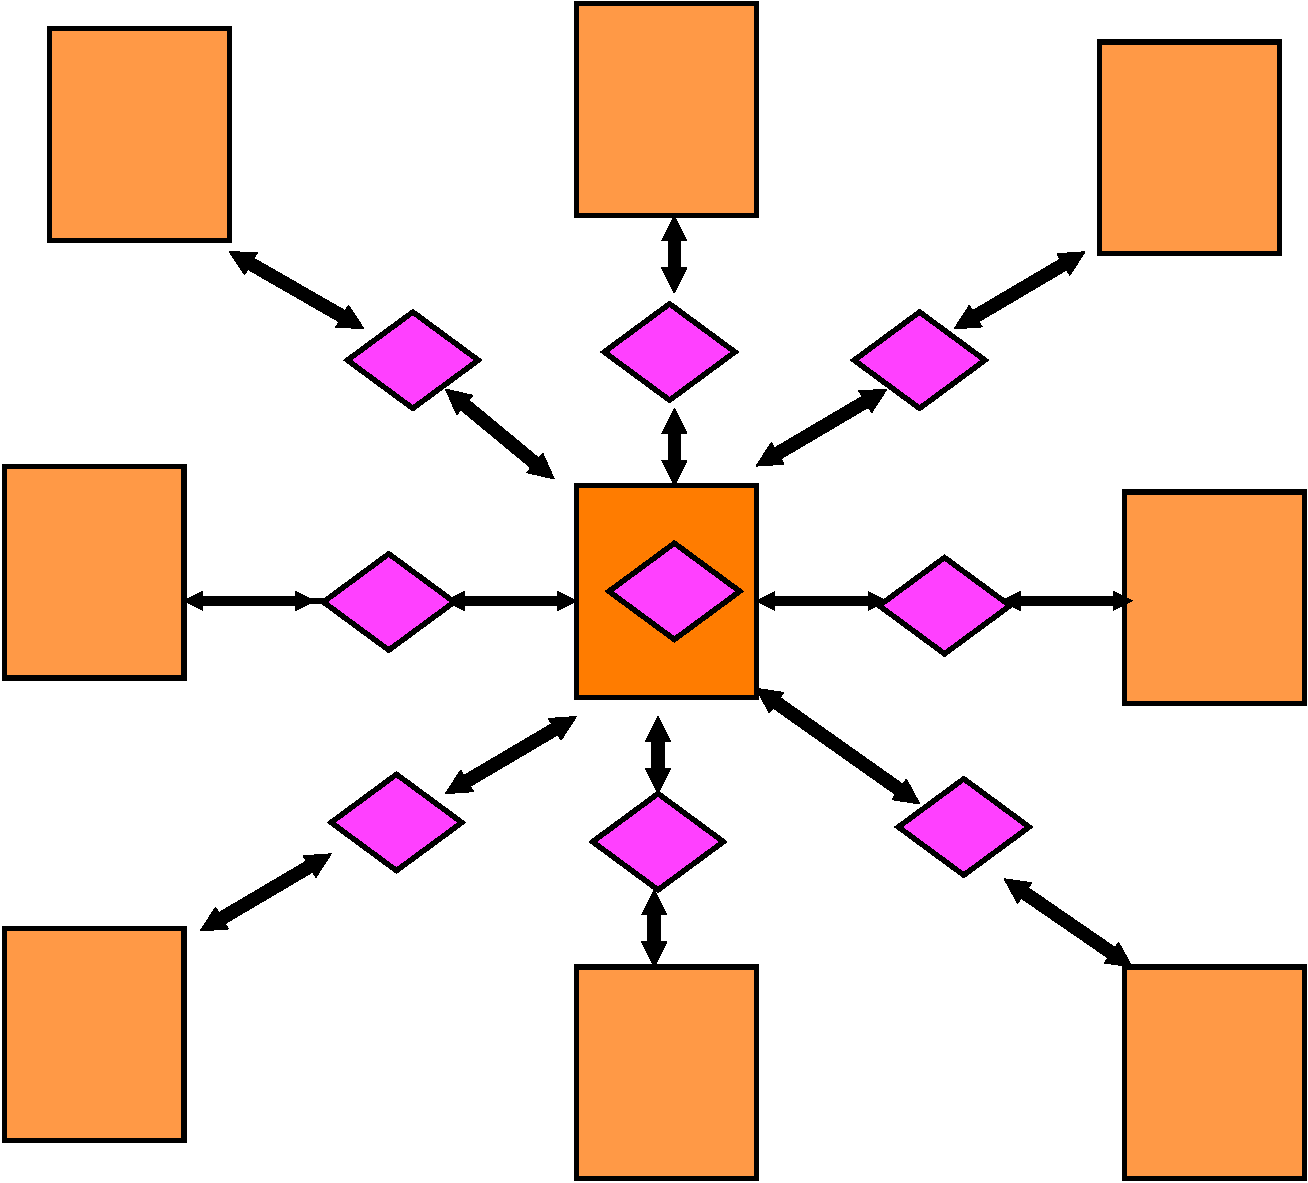
\includegraphics[width=0.8\textwidth]{figures/namd_decomp2.pdf} \end{center}
  \column{.6\textwidth}
  \begin{itemize}
    \item Now, we have many objects to load balance:
    \begin{itemize}
      \item Each diamond can be  assigned to any proc.
      \item Number of diamonds (3D): 14*Number of Patches
    \end{itemize}
    \pause
    \item 2-away variation:
    \begin{itemize}
      \item Half-size cubes
      \item Communicate only with neighbors
      \item 5 x 5 x 5 interactions
    \end{itemize}
    \pause
    \item 3-away interactions: 7 x 7 x 7
  \end{itemize}
  \end{columns}
\end{frame}

\begin{frame}[t]
\frametitle{NAMD Parallelization Using Charm++}
The computation is decomposed into ``natural'' objects of the application, which
are assigned to processors by Charm++ RTS
  \begin{center} 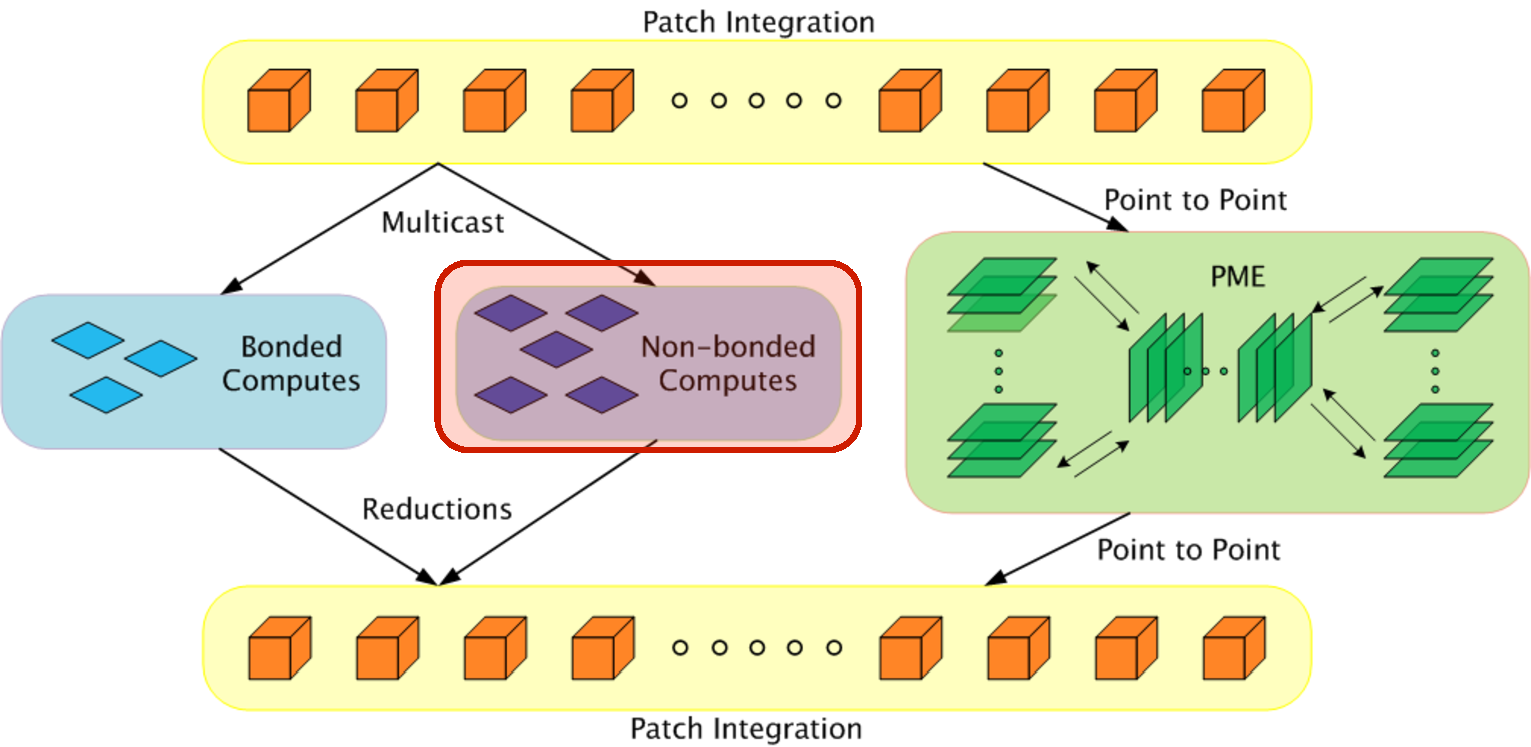
\includegraphics[width=\textwidth]{figures/md_parallelize.pdf} \end{center}
\end{frame}

\begin{frame}[t]
\frametitle{NAMD Projections}
  \begin{center} 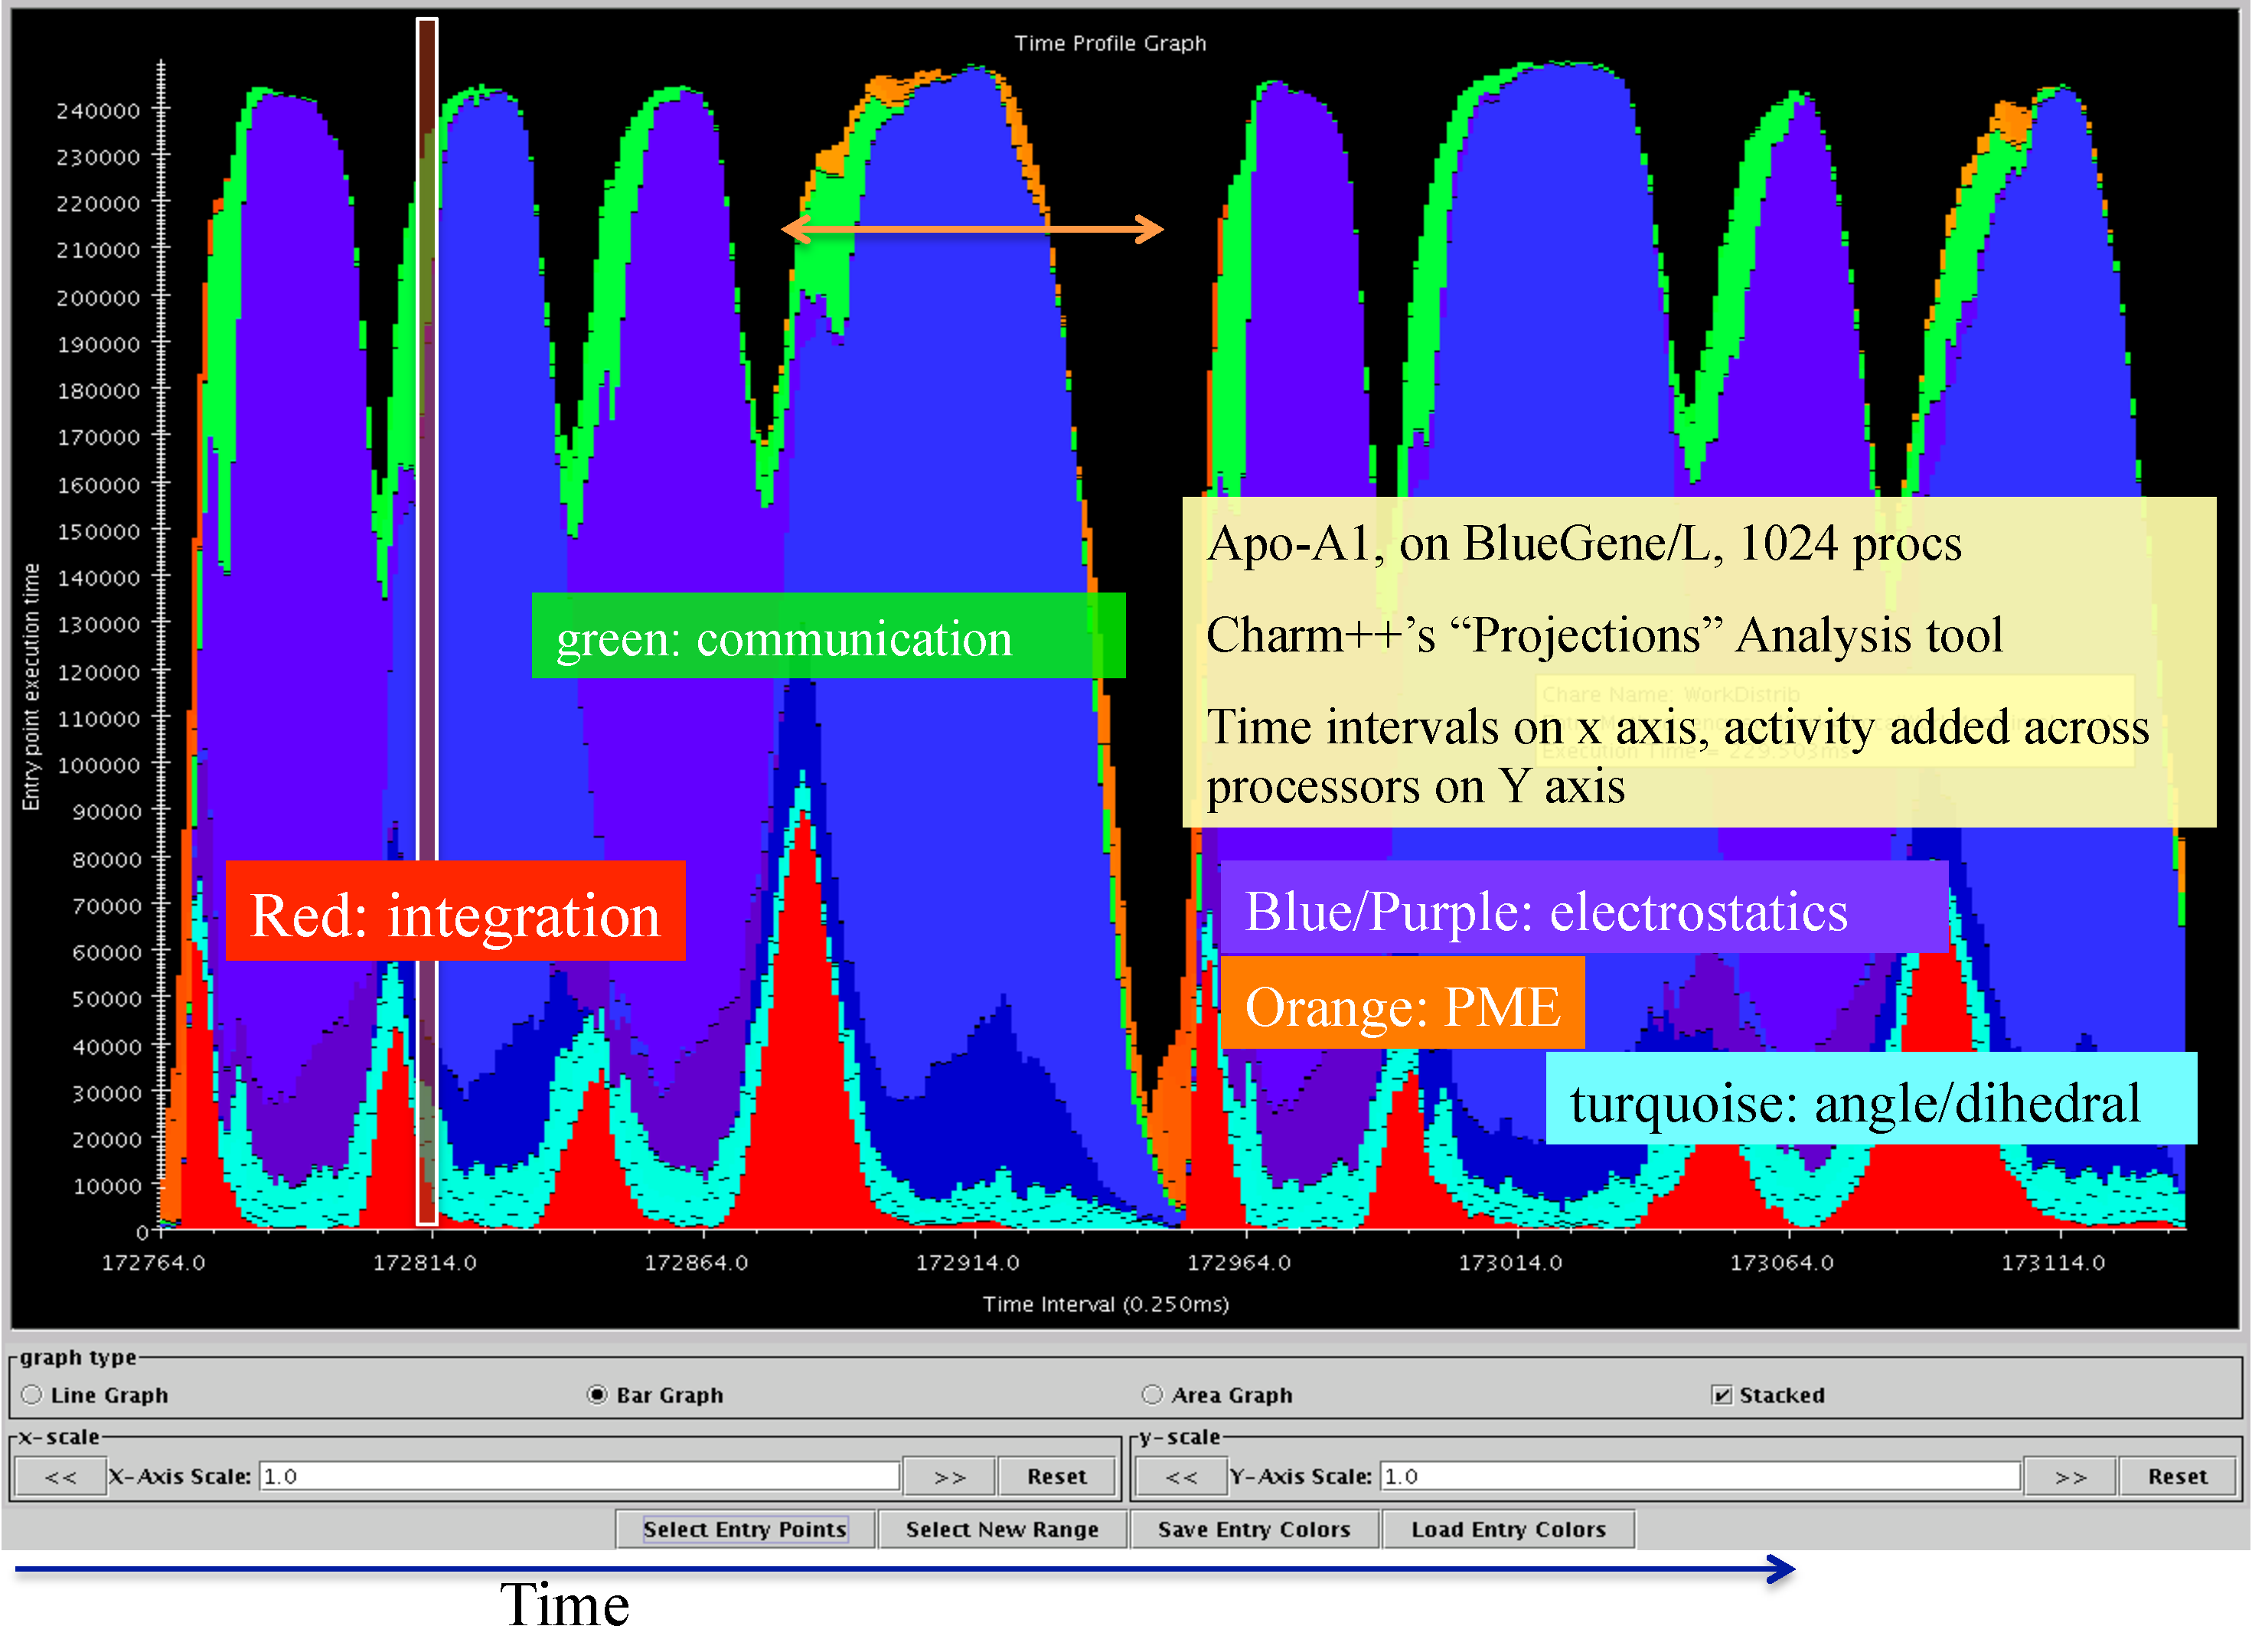
\includegraphics[width=.9\textwidth]{figures/namd_projection.pdf} \end{center}
\end{frame}

\begin{frame}[t]
\frametitle{DHFR Performance on Titan}
  \begin{itemize}
  \item Best performance is 590us/step
  \end{itemize}
  \begin{center} 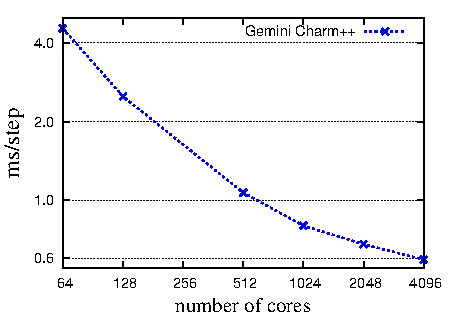
\includegraphics[width=.8\textwidth]{figures/jac-titan-pme4.pdf} \end{center}
\end{frame}

\begin{frame}[t]
\frametitle{Apoa1 Performance on BG/P BG/Q}
  \begin{itemize}
  \item Best performance on BG/Q is 794us/step
  \end{itemize}
  \begin{center} 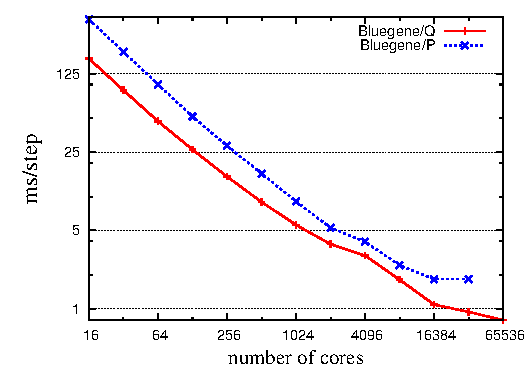
\includegraphics[width=.8\textwidth]{figures/apoa1-pme4-PQ.pdf} \end{center}
\end{frame}

\begin{frame}[t]
\frametitle{NAMD Performance on IBM Blue Gene/P}
  \begin{center} 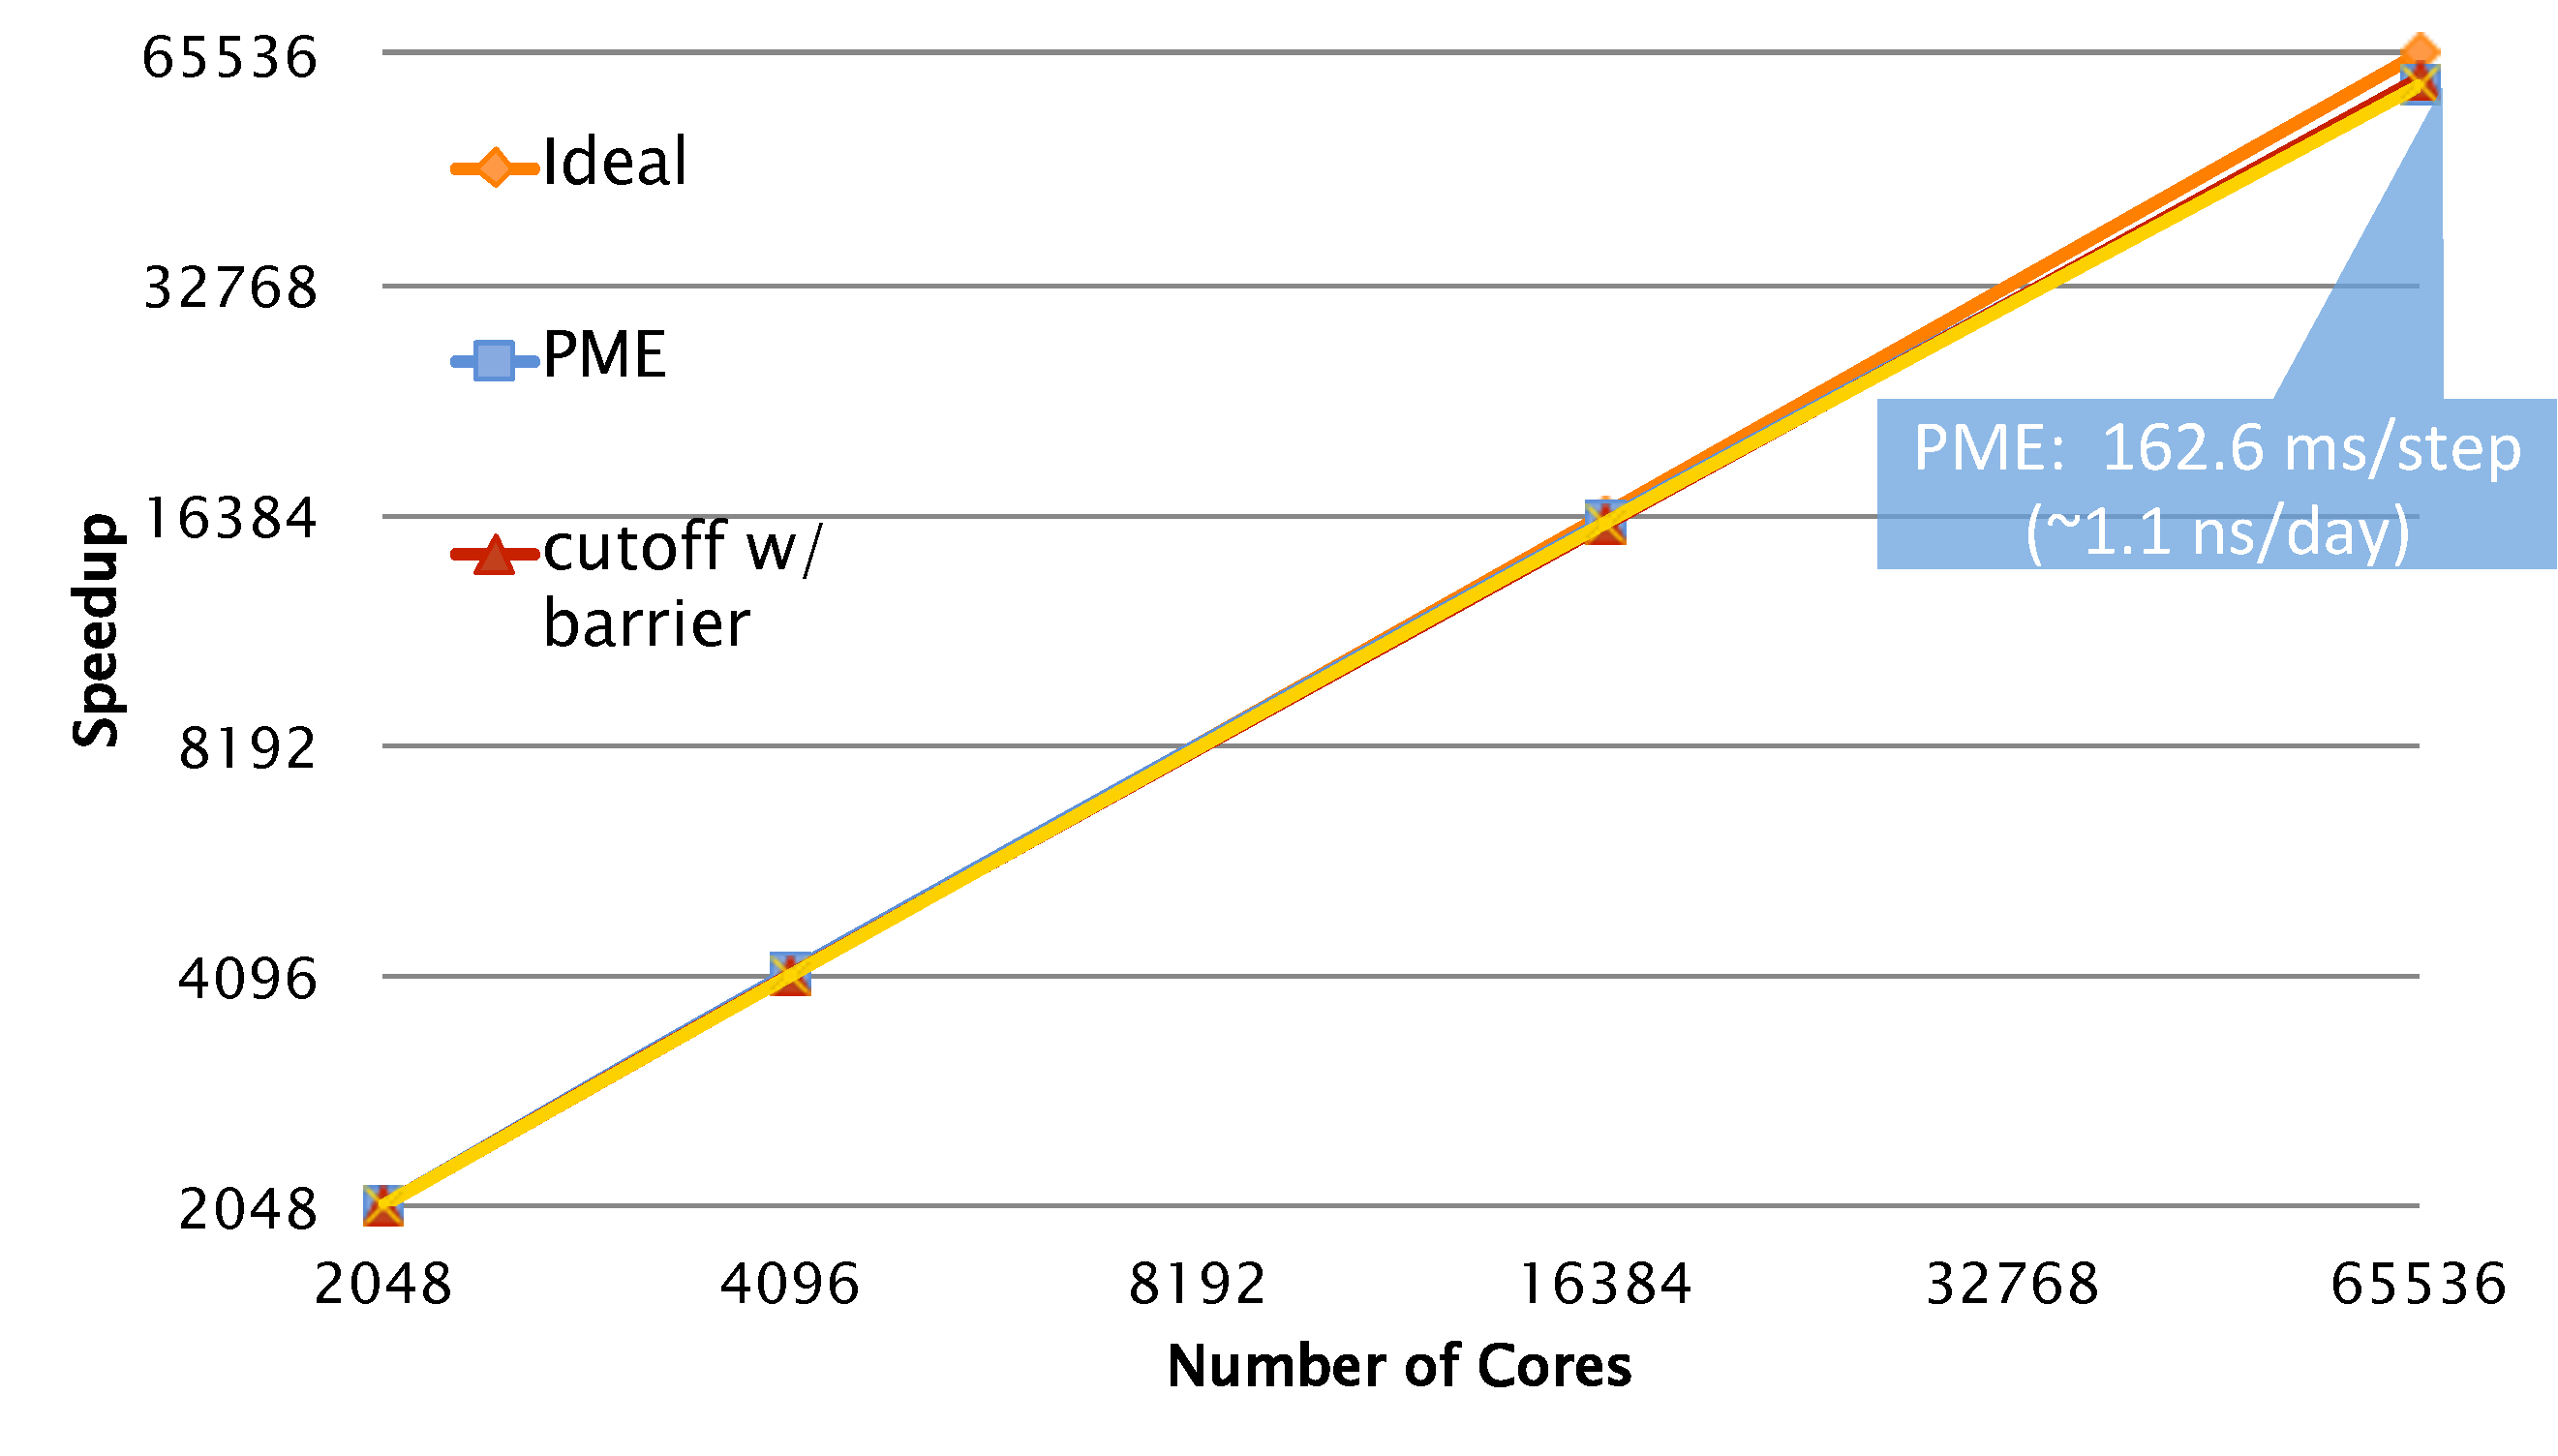
\includegraphics[width=.8\textwidth]{figures/namd_bgp.pdf} \end{center}
\end{frame}

\begin{frame}[t]
\frametitle{100M STMV Performance on Titan}
  \begin{center} 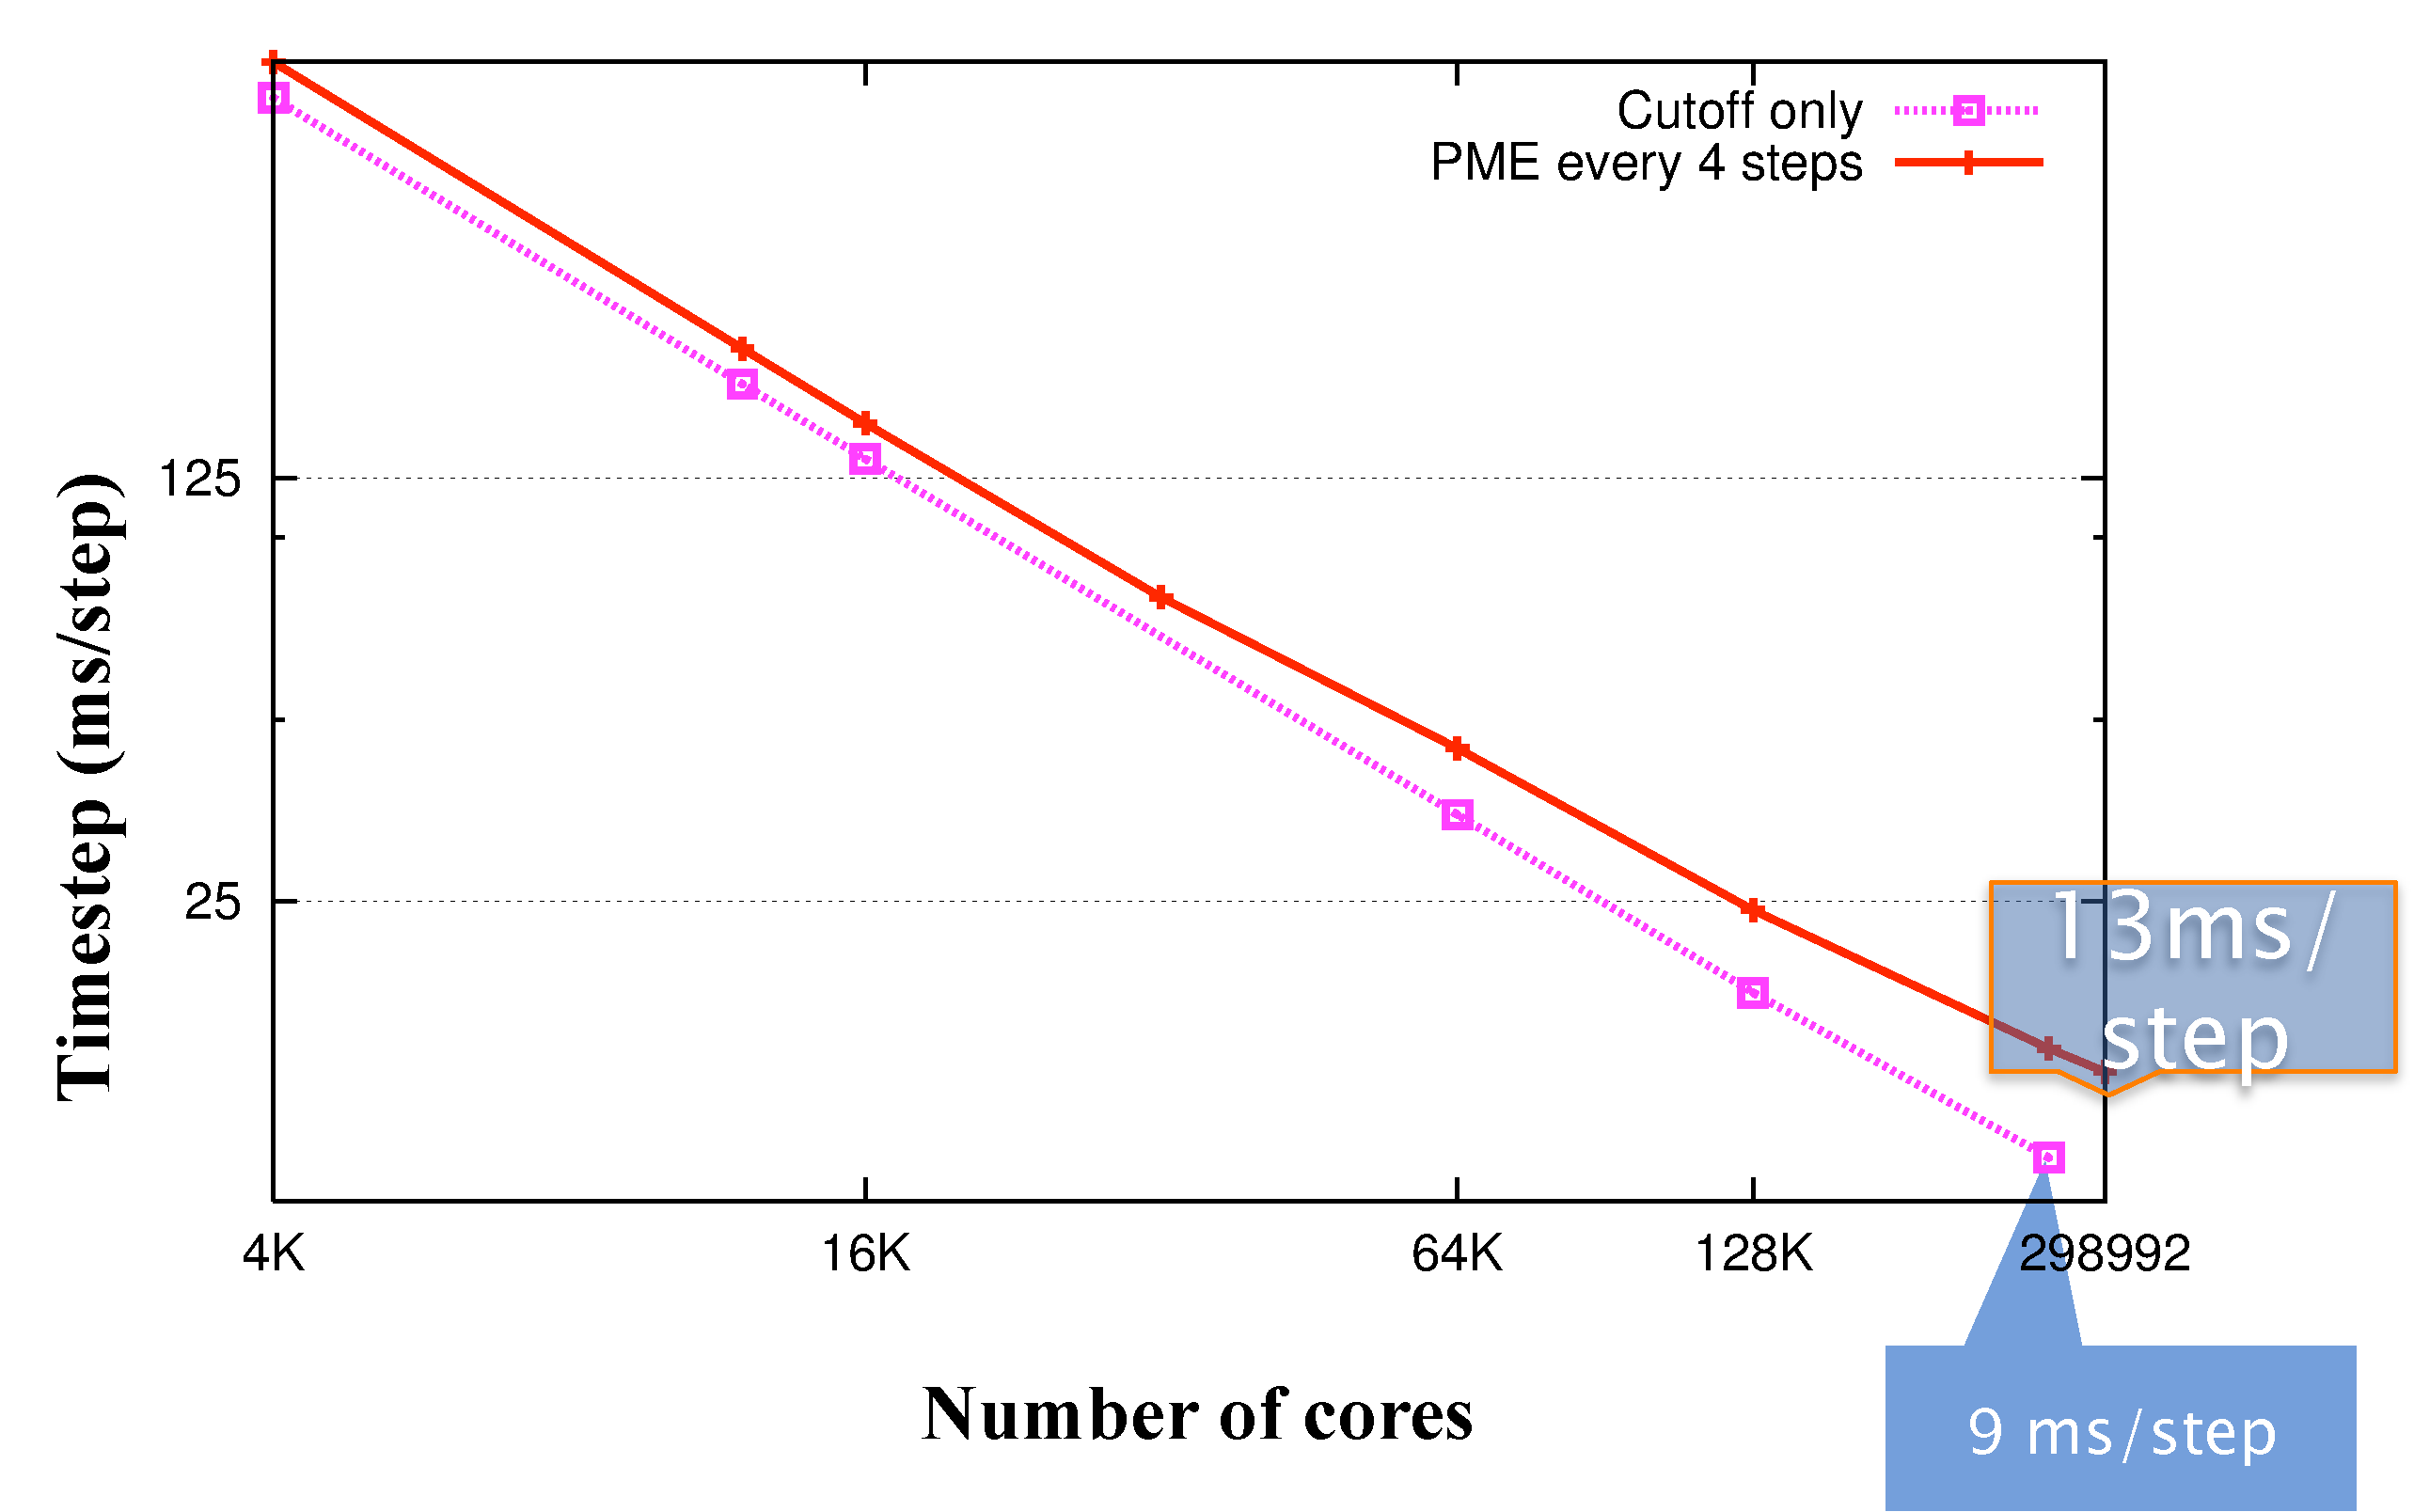
\includegraphics[width=.8\textwidth]{figures/namd_titan.pdf} \end{center}
\end{frame}

\begin{frame}[t]
\frametitle{ChaNGa: Parallel Gravity}
  \begin{itemize}
    \item Collaborative project (NSF)
    \begin{itemize} 
        \item with Tom Quinn, Univ. of Washington
    \end{itemize}
    \pause
    \item Evolution of Universe and Galaxy Formation
    \item Gravity, gas dynamics
    \pause
    \item Barnes-Hut tree codes
    \begin{itemize} 
      \item Oct tree is natural decomposition
      \item Geometry has better aspect ratios, so you ``open” up fewer nodes
      \item But is not used because it leads to bad load balance
      \item Assumption: one-to-one map between sub-trees and PEs
      \item Binary trees are considered better load balanced
    \end{itemize}
    \pause
    \item With Charm++: Use Oct-Tree, and let Charm++ map subtrees to processors
  \end{itemize}
\end{frame}

\begin{frame}[t]
\frametitle{ChaNGa: Control Flow}
  \begin{center} 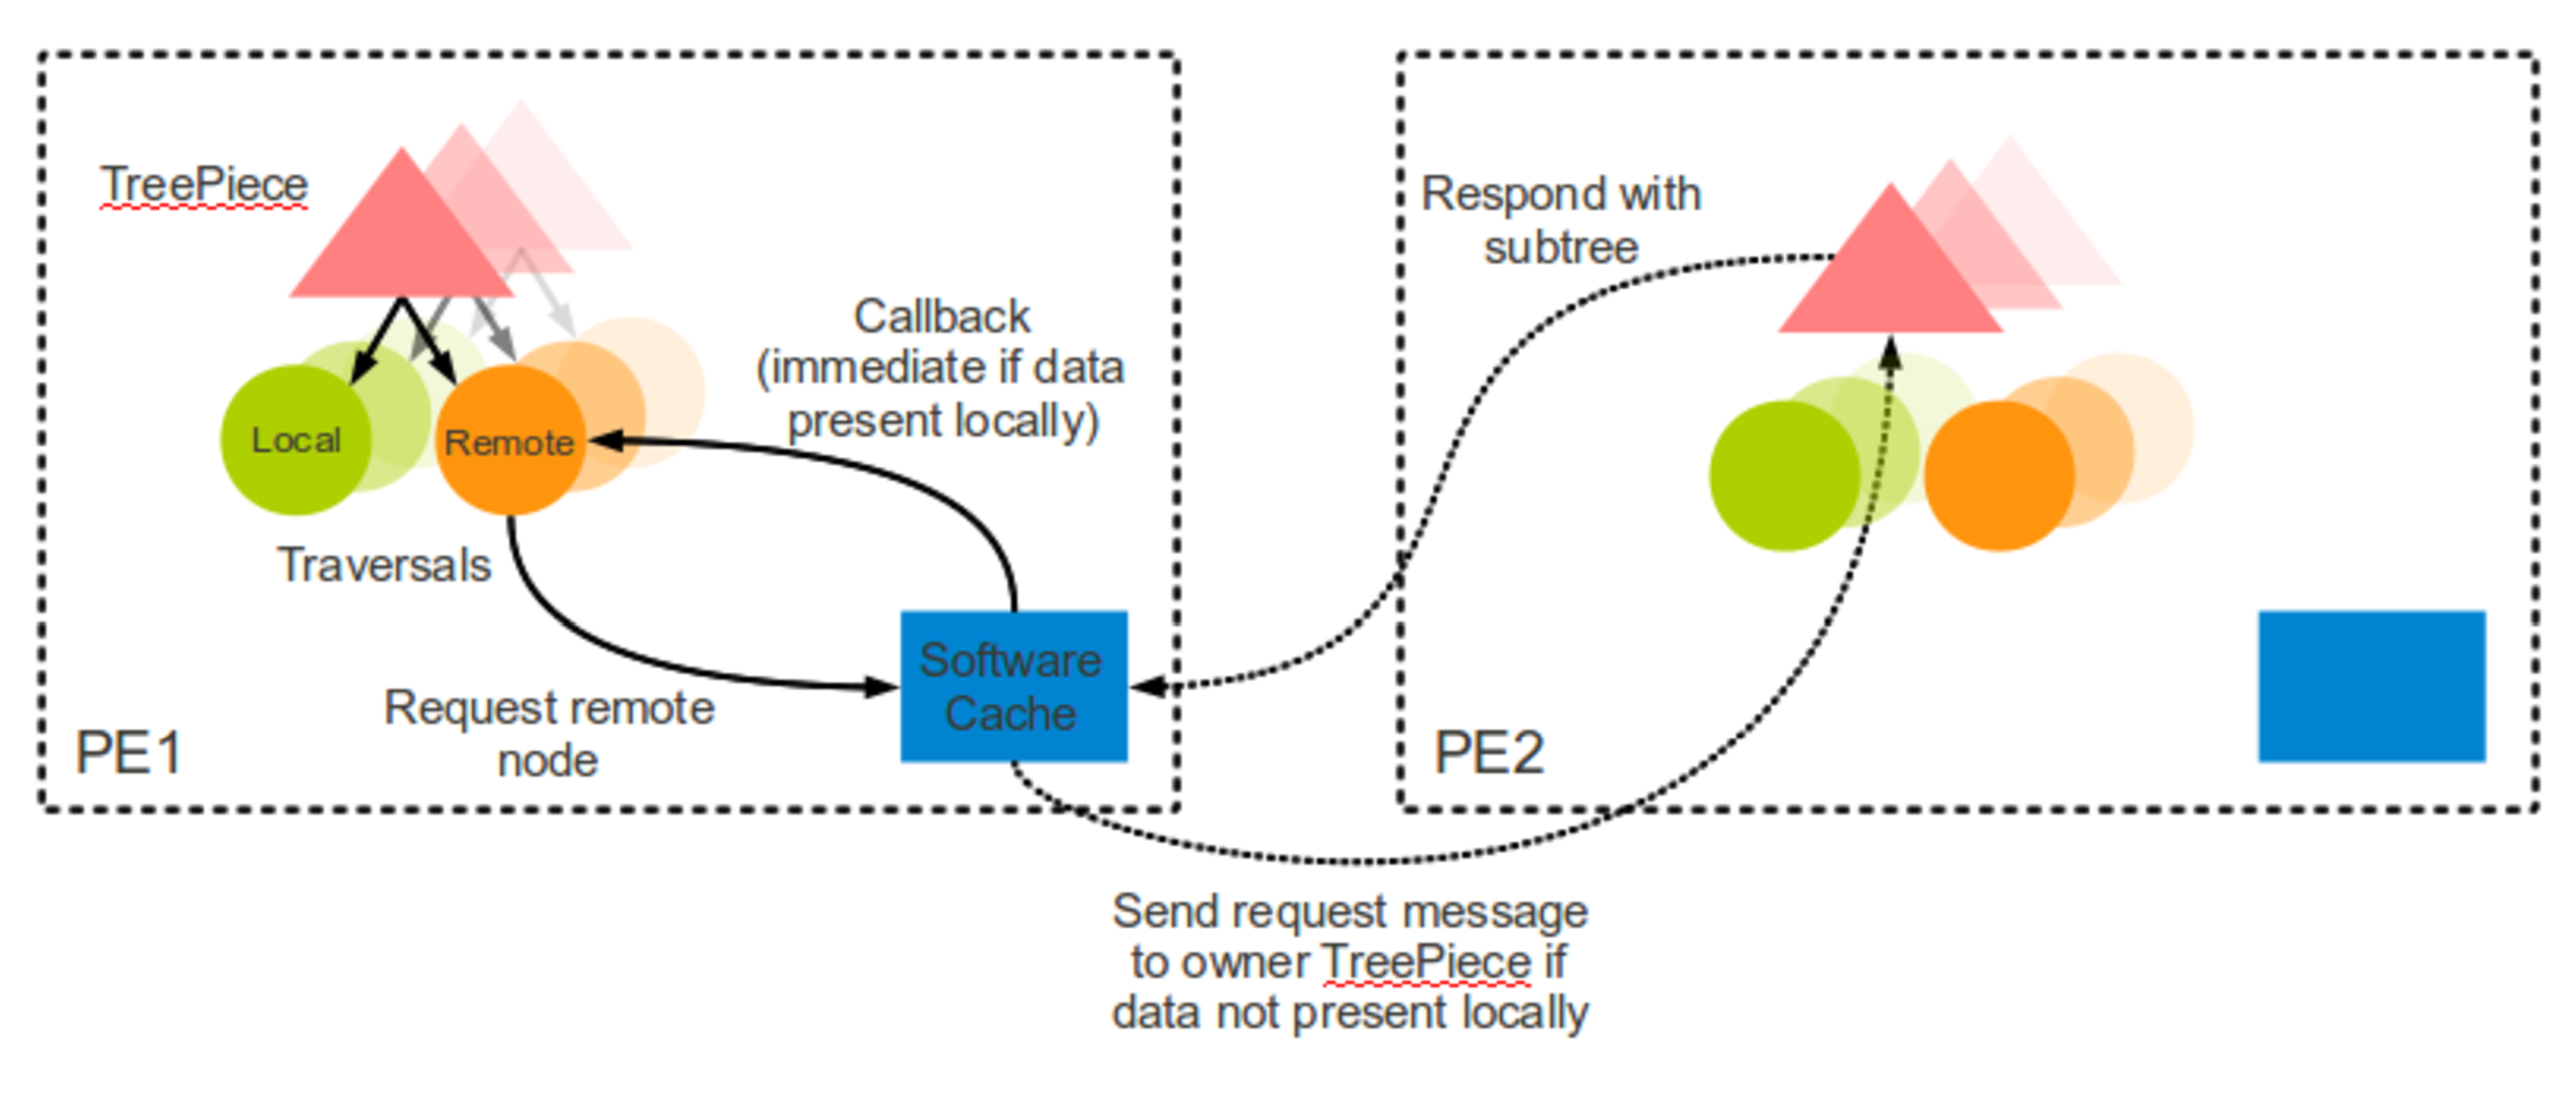
\includegraphics[width=\textwidth]{figures/changa.pdf} \end{center}
\end{frame}

\begin{frame}[t]
\frametitle{OpenAtom: MD with quantum effects}
  \begin{columns}
  \column{.5\textwidth}
    \begin{itemize}
      \item Much more fine-grained:
      \begin{itemize}
        \item Each electronic state is modeled with a large array
      \end{itemize}
      \pause
      \item Collaboration with:
      \begin{itemize}
        \item G. Martyna (IBM) 
        \item M. Tuckerman (NYU)
      \end{itemize}
      \pause
    \item Using Charm++ virtualization, we can efficiently scale small (32 molecule) systems to thousands of processors
  \end{itemize}
  \column{.5\textwidth}
  \begin{center} 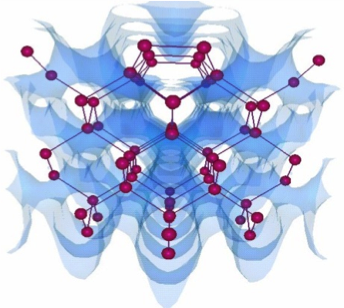
\includegraphics[width=.5\textwidth]{figures/openatom1.png}\\
  \textcolor{red}{Semiconductor Surfaces}\end{center}
  \begin{center} 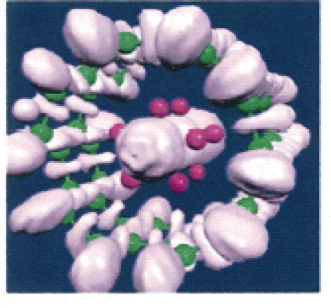
\includegraphics[width=.5\textwidth]{figures/openatom2.png}\\
  \textcolor{red}{Nanowires}\end{center}
  \end{columns}
\end{frame}


\begin{frame}[t]
\frametitle{OpenAtom: Decomposition and Computation Flow}
  \begin{center} 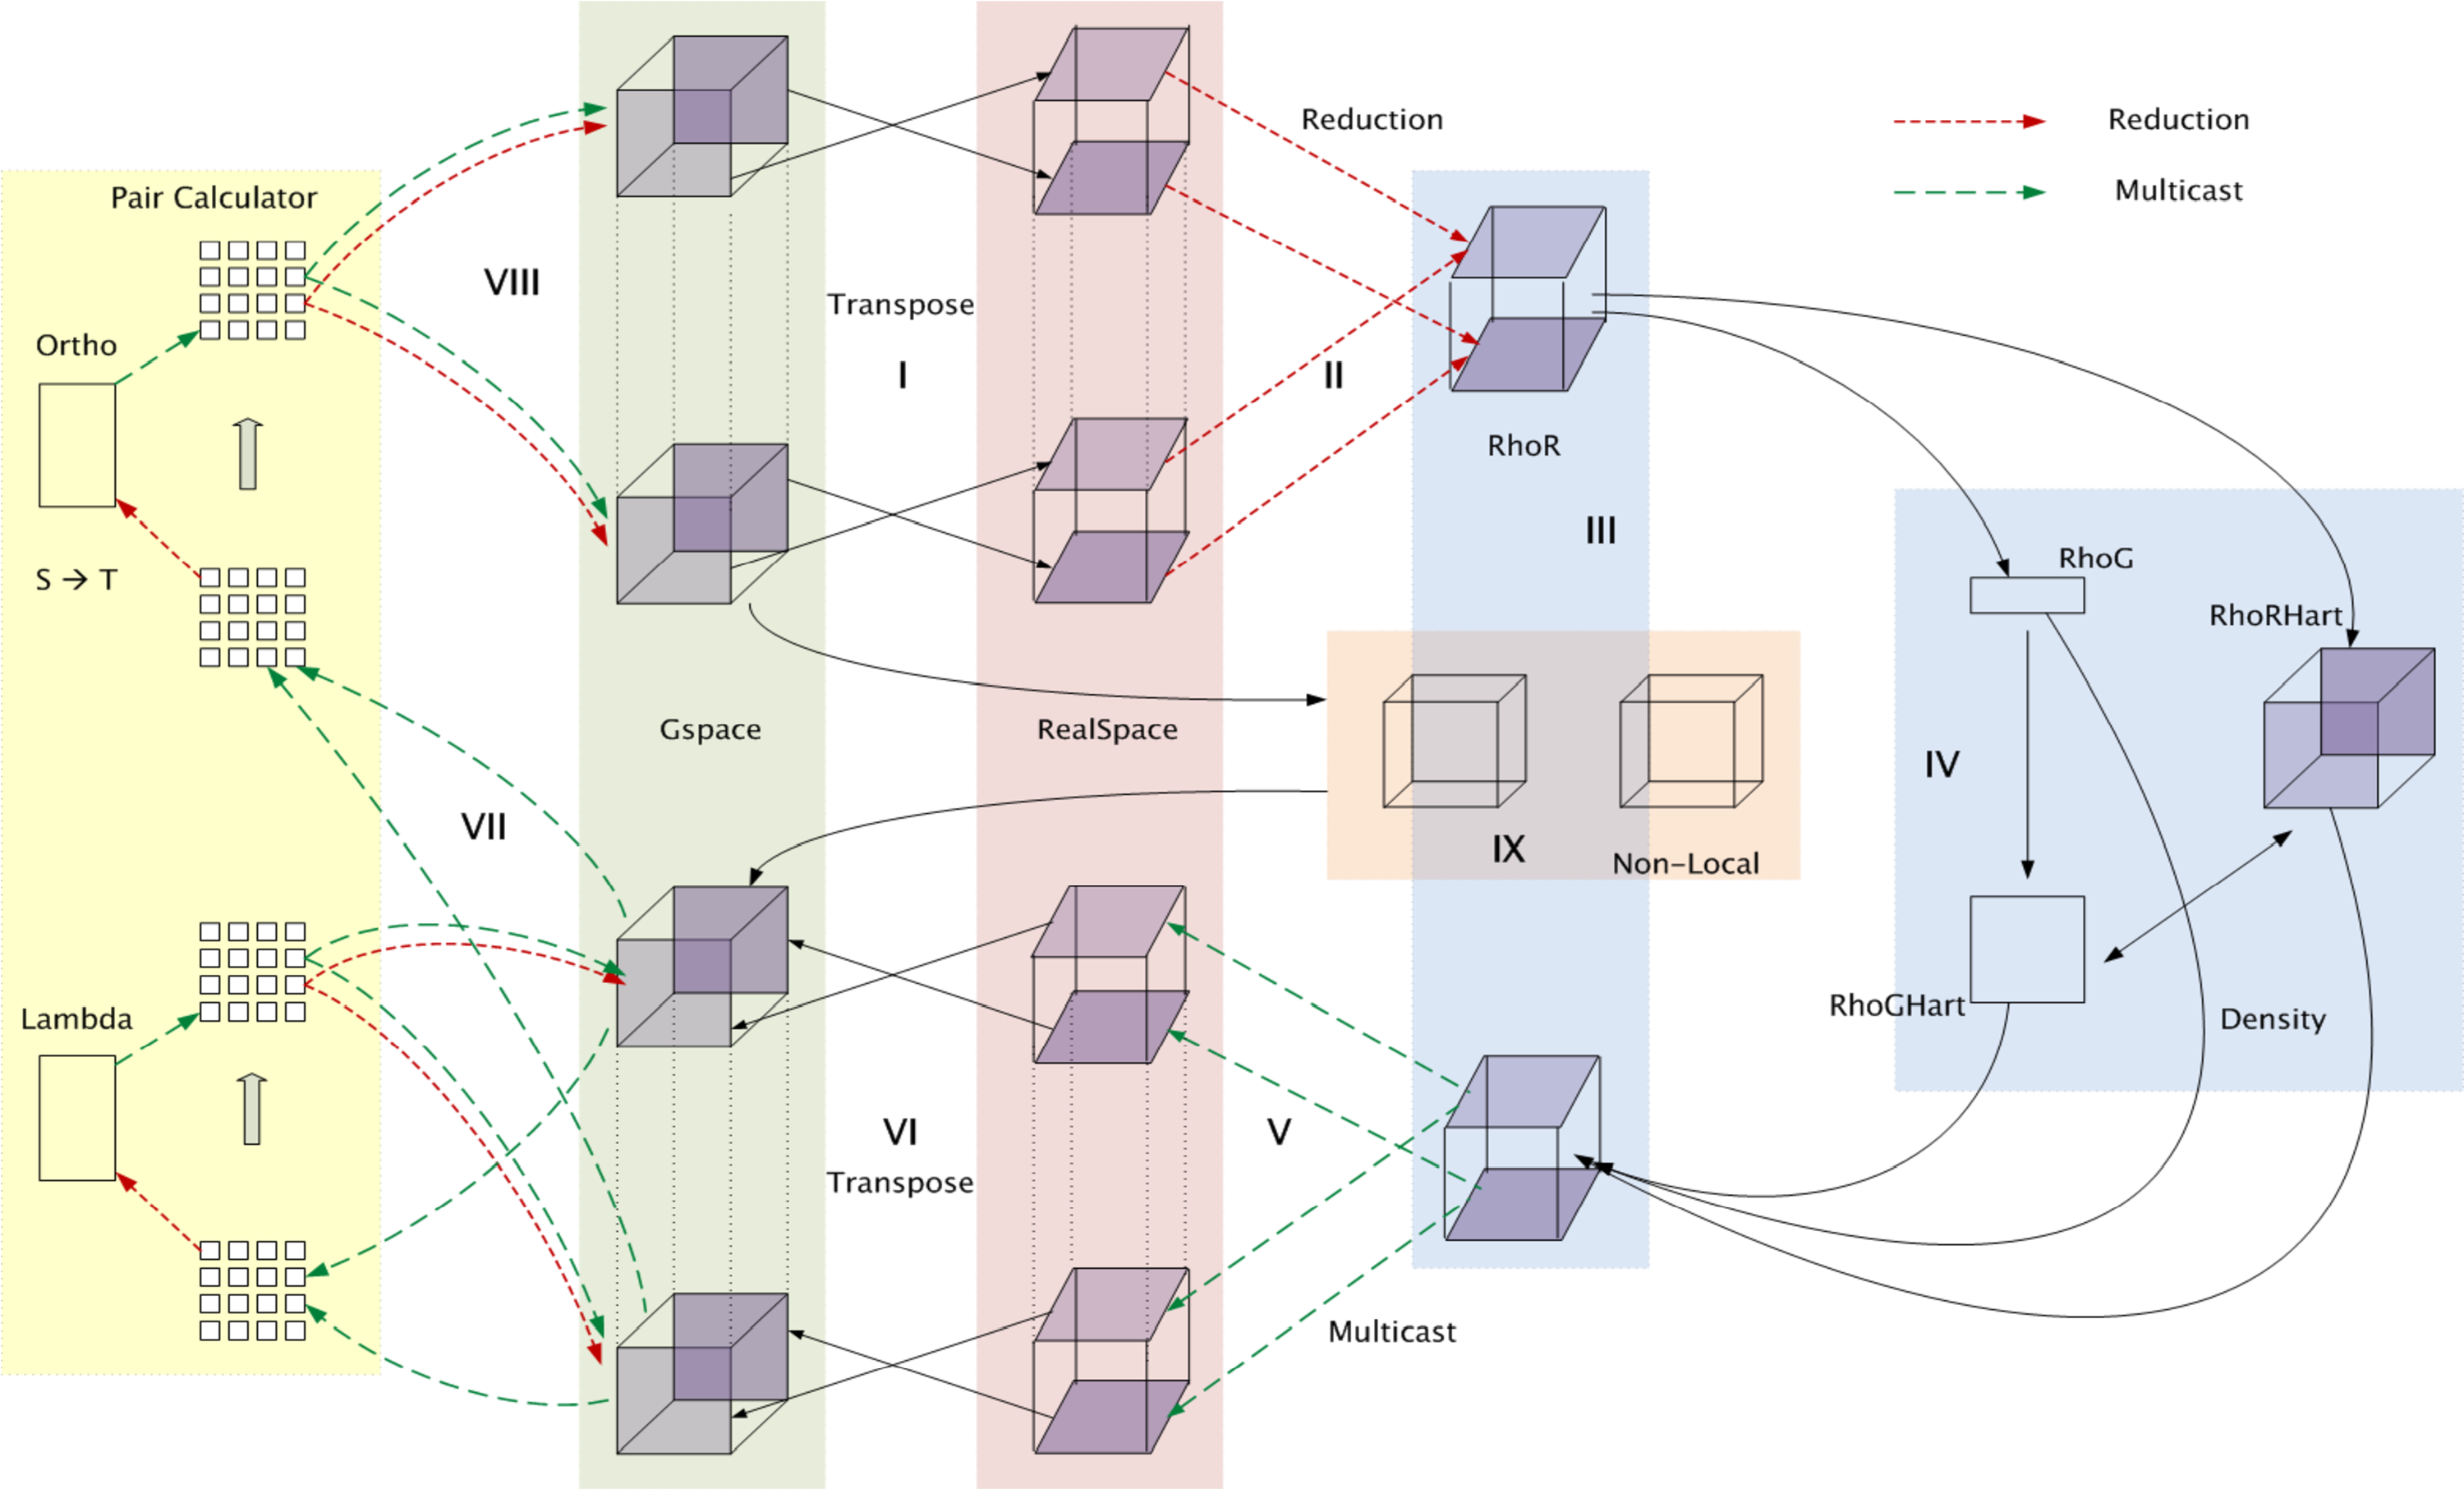
\includegraphics[width=\textwidth]{figures/openatom_array.pdf} \end{center}
\end{frame}

% \begin{frame}[t]
% \frametitle{OpenAtom: Topology Aware Mapping of Objects}
%   \begin{center} 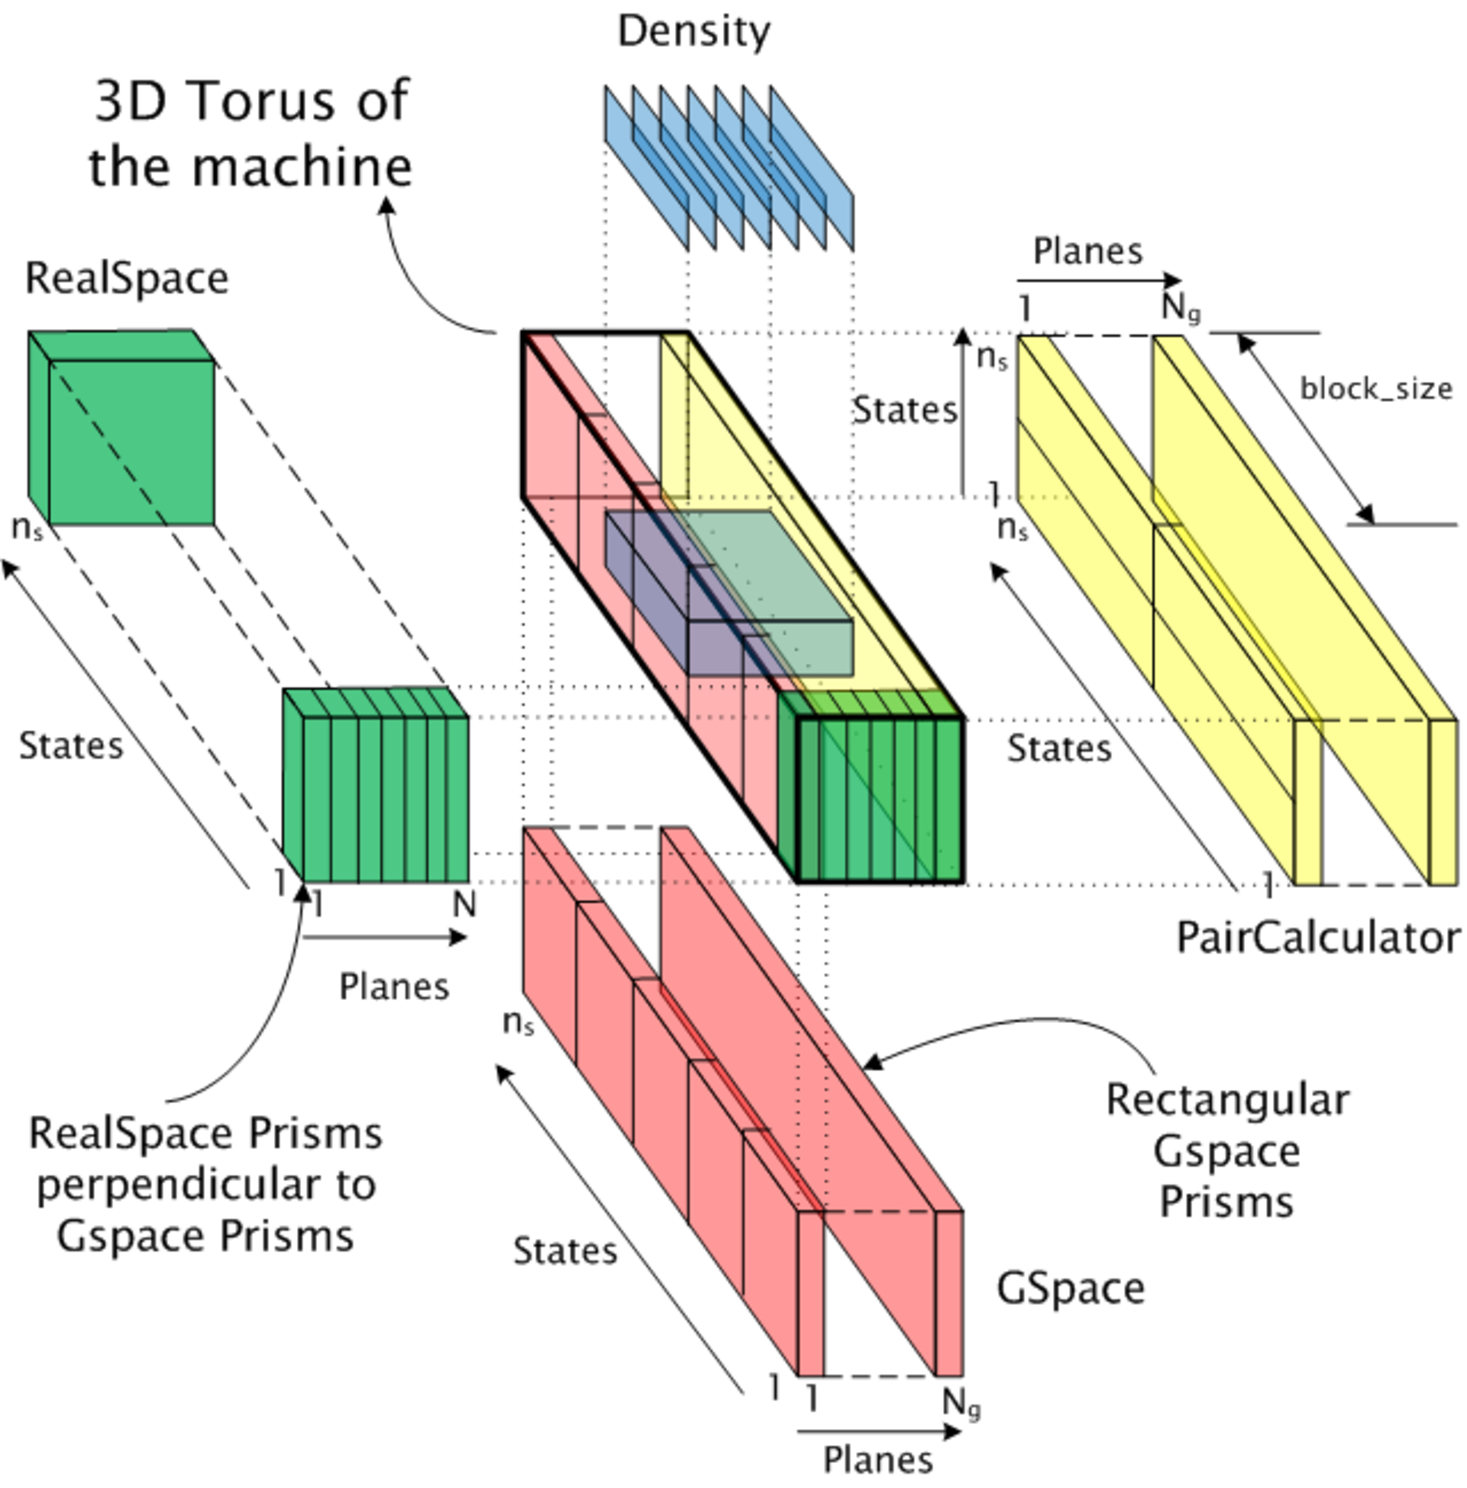
\includegraphics[width=.45\textwidth]{figures/openatom_topo.pdf} \end{center}
%   Object based decomposition provides new degrees of freeedom to easily try
%   different mappings of objects to processors, to help minimize contention

% \end{frame}
